\Large\textbf{}\\
\Large\textbf{Use Case X Creazione Oggetto} \\
\vspace{0.5cm}
%\begin{figure}[h]
%  \centering
%  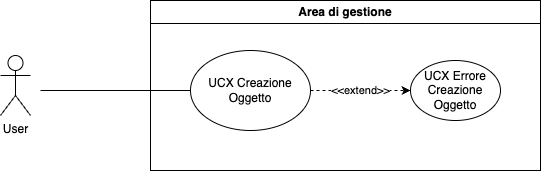
\includegraphics[width=0.8\textwidth]{UseCasesImages/ObjCr.png}
%\end{figure}

\large\textbf{} \\
\textbf{Attori:} User\\
\textbf{Pre-condizione:} Magazzino correttamente istanziato \\
\textbf{Post-condizione: } Creazione Oggetto\\
\textbf{Scenario Principale:}  L'utente crea un oggetto inserendone le \textit{specifiche caratteristiche}. Se i dati inseriti non rispettano il \textit{criterio prestabilito} viene visualizzato un messaggio di errore.\\
\textbf{Estensioni: } UCX Errore Creazione Oggetto\\

\vspace{0.5cm}

\textbf{}\\
{\color{red}{\textbf{Domanda:} Un oggetto puó essere creato e memorizzato in uno spazio apposito senza essere inserito in una scaffalatura o la creazione coincide con l'inserimento?}} \\
{\color{red}{\textbf{Domanda:} Quali sono le caratteristiche di un oggetto? In particolare: \\-Un oggetto puó superare i limiti di dimensione di una scaffalatura? \\ -Gli oggetti hanno forma standardizzata?}}\\

\vspace{0.5cm}

\Large\textbf{}\\
\Large\textbf{Use Case X Errore Creazione Oggetto} \\
\large\textbf{} \\
\textbf{Attori:} User\\
\textbf{Pre-condizione:} L'utente ha inserito dati scorretti nella schermata di creazione di un oggetto\\
\textbf{Post-condizione: } Visualizzazione Errore\\
\textbf{Scenario Principale:} Il sistema mostra a schermo un messaggio contenente le specifiche dell'errore di inserimento\\

\vspace{0.5cm}

\Large\textbf{}\\
\Large\textbf{Use Case X Ricerca Statica Oggetto} \\
\vspace{0.5cm}
%\begin{figure}[h]
%  \centering
%  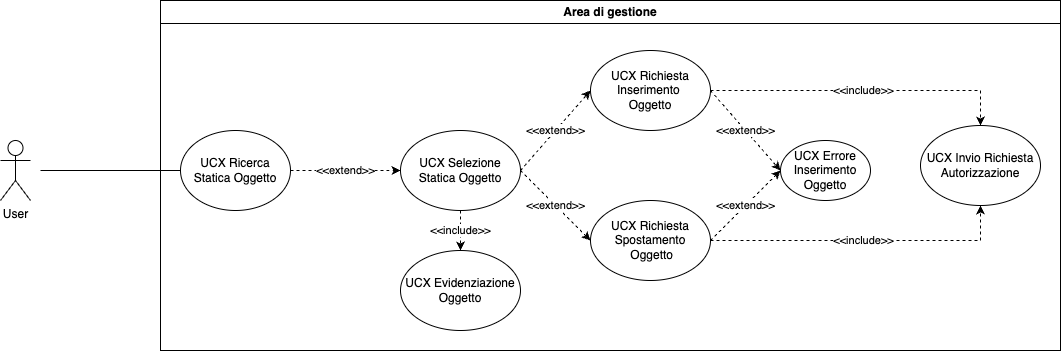
\includegraphics[width=0.8\textwidth]{UseCasesImages/StaticRes.png}
%\end{figure}

\large\textbf{} \\
\textbf{Attori:} User\\
\textbf{Pre-condizione:} Magazzino correttamente istanziato, l'user si ritrova nell'area di gestione \\
\textbf{Post-condizione: } Visualizzazione lista oggetti corrispondenti a dati inseriti\\
\textbf{Scenario Principale:}  L'utente effettua una ricerca seguendo dei particolari \textit{parametri} e il sistema ritorna una lista (anche vuota) di oggetti corrispondenti. Sará poi possibile selezionare gli oggetti\\
\textbf{Estensione:} UCX Selezione Statica Oggetto

\textbf{}\\
{\color{red}{\textbf{Domanda:} Quali sono i parametri di ricerca degli oggetti?}}\\

\vspace{0.5cm}

\Large\textbf{}\\
\Large\textbf{Use Case X Selezione Statica Oggetto} \\
%\begin{figure}[h]
%  \centering
%  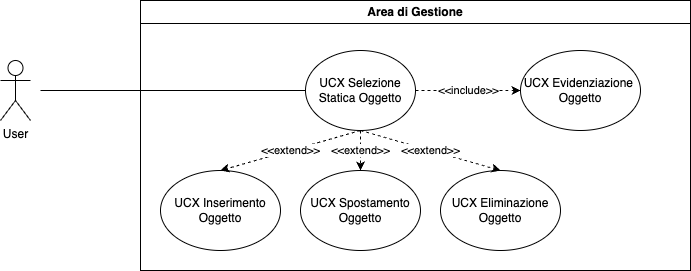
\includegraphics[width=0.8\textwidth]{UseCasesImages/StaticSel.png}
%\end{figure}

\vspace{0.5cm}

\large\textbf{} \\
\textbf{Attori:} User\\
\textbf{Pre-condizione:} L'user si trova nell'area di gestione e sta visualizzando una lista di oggetti \\
\textbf{Post-condizione: } Selezione di un oggetto e relativa evidenziazione\\
\textbf{Scenario Principale:}  L'utente sceglie uno degli oggetti presenti in una lista e, se giá inserito in una scaffalatura, l'oggetto selezionato viene evidenziato nell'ambiente tridimensionale. Una volta selezionato un oggetto sará possibile inserirlo (se non precedentemente inserito), spostarlo o eliminarlo.\\
\textbf{Inclusione:} UCX Evidenziazione Oggetto \\
\textbf{Estensioni:} \\ 
-UCX Inserimento oggetto \\ -UCX Spostamento Oggetto \\ -UCX Eliminazione Oggetto

\vspace{0.5cm}

\Large\textbf{}\\
\Large\textbf{Use Case X Evidenziazione Oggetto} \\

\large\textbf{} \\
\textbf{Attori:}\\
\textbf{Pre-condizione:} Un oggetto presente nel magazzino é stato selezionato \\
\textbf{Post-condizione: } Evidenziazione dell'oggetto selezionato \\
\textbf{Scenario Principale:}  Se l'oggetto selezionato é presente nel magazzino esso viene evidenziato nello spazio tridimensionale\\

\vspace{0.5cm}
\newpage

\Large\textbf{}\\
\Large\textbf{Use Case X Selezione 3D Oggetto} \\
%\begin{figure}[h]
%  \centering
%  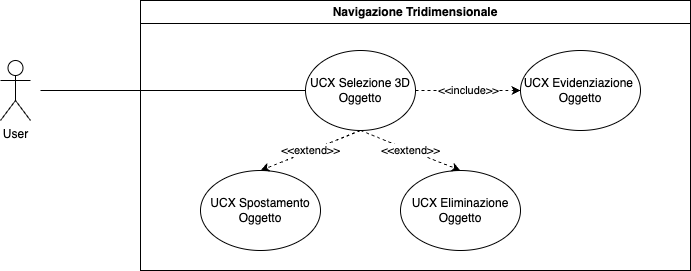
\includegraphics[width=0.8\textwidth]{UseCasesImages/3DSel.png}
%\end{figure}

\vspace{0.5cm}

\large\textbf{} \\
\textbf{Attori:} User\\
\textbf{Pre-condizione:} L'user si trova nell'area di navigazione tridimensionale \\
\textbf{Post-condizione: } Selezione di un oggetto e relativa evidenziazione\\
\textbf{Scenario Principale:}  Navigando nello spazio tridimensionale l'utente seleziona un oggetto che viene conseguentemente evidenziato; una volta selezionato sará possibile spostarlo o eliminarlo.\\
\textbf{Inclusione:} UCX Evidenziazione Oggetto \\
\textbf{Estensioni:} \\ 
-UCX Spostamento Oggetto \\ -UCX Eliminazione Oggetto

\vspace{0.5cm}


\Large\textbf{}\\
\Large\textbf{Use Case X Inserimento Oggetto} \\
%\begin{figure}[h]
% \centering
%  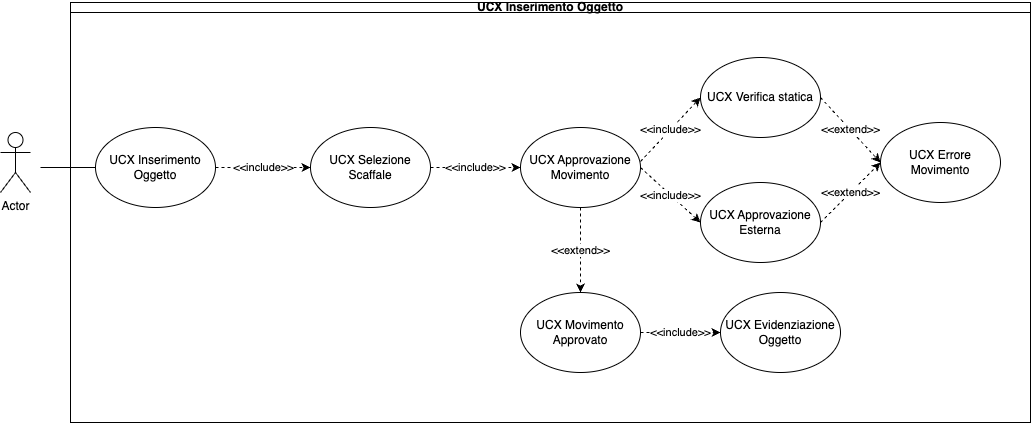
\includegraphics[width=0.8\textwidth]{UseCasesImages/Inserimento.png}
%\end{figure}

\vspace{0.5cm}

\large\textbf{} \\
\textbf{Attori:} User\\
\textbf{Pre-condizione:} L'utente ha selezionato un oggetto  \\
\textbf{Post-condizione: } L'oggetto é stato inserito correttamente oppure viene visualizzato un messaggio di errore\\
\textbf{Scenario Principale:}  Dopo aver selezionato un oggetto l'utente ha scelto di inserirlo nel magazzino, sceglie uno scaffale a cui destinarlo e vengono effettuate una serie di verifiche. La prima verifica effettuata é di natura statica: il sistema verifica la disponibilitá dimensionale del magazzino. Dopo aver passato la verifica statica la richiesta di spostamento viene inoltrata ad un gestore incaricato di approvare il movimento o rifiutarlo. In caso il movimento non venga effettuato viene visualizzato un messaggio di errore \\
\textbf{Inclusione:} UCX Selezione Scaffale \\

\vspace{0.5cm}

\Large\textbf{}\\
\Large\textbf{Use Case X Spostamento Oggetto} \\
%\begin{figure}[h]
%  \centering
%  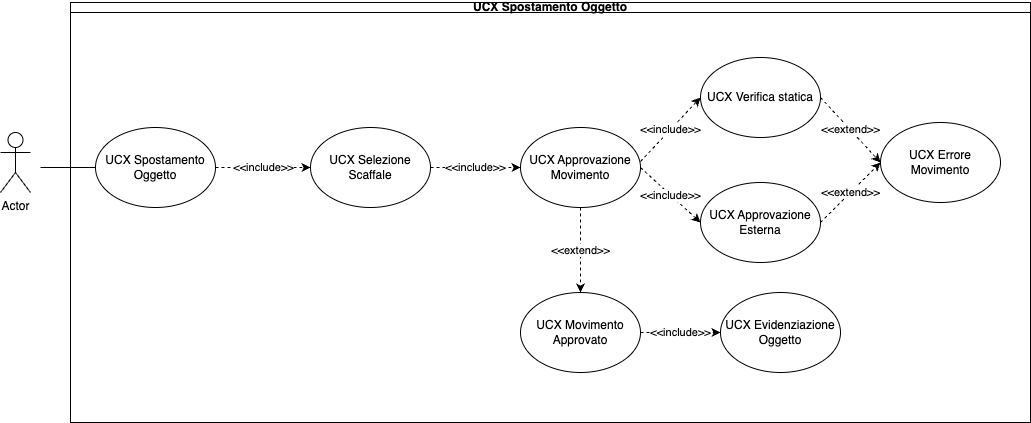
\includegraphics[width=0.8\textwidth]{UseCasesImages/Spostamento.png}
%\end{figure}

\vspace{0.5cm}

\large\textbf{} \\
\textbf{Attori:} User\\
\textbf{Pre-condizione:} L'utente ha selezionato un oggetto  \\
\textbf{Post-condizione: } L'oggetto é stato spostato correttamente oppure viene visualizzato un messaggio di errore\\
\textbf{Scenario Principale:}  Dopo aver selezionato un oggetto l'utente ha scelto di spostarlo, sceglie uno scaffale a cui destinarlo e vengono effettuate una serie di verifiche. La prima verifica effettuata é di natura statica: il sistema verifica la disponibilitá dimensionale del magazzino. Dopo aver passato la verifica statica la richiesta di spostamento viene inoltrata ad un gestore incaricato di approvare il movimento o rifiutarlo. In caso il movimento non venga effettuato viene visualizzato un messaggio di errore \\
\textbf{Inclusione:} UCX Selezione Scaffale \\

\vspace{0.5cm}

\Large\textbf{}\\
\Large\textbf{Use Case X Eliminazione Oggetto} \\

\vspace{0.5cm}

\large\textbf{} \\
\textbf{Attori:} User\\
\textbf{Pre-condizione:} L'utente ha selezionato un oggetto  \\
\textbf{Post-condizione: } L'oggetto é eliminato\\
\textbf{Scenario Principale:}  Dopo aver selezionato un oggetto l'utente ha scelto di eliminarlo \\

\vspace{0.5cm}

\Large\textbf{}\\
\Large\textbf{Use Case X Approvazione Movimento} \\

\vspace{0.5cm}

\large\textbf{} \\
\textbf{Attori:} User\\
\textbf{Pre-condizione:} L'utente ha selezionato un oggetto e uno scaffale a cui destinarlo \\
\textbf{Post-condizione: } Il movimento é stato effettuato correttamente o viene visualizzato un messaggio di errore\\
\textbf{Scenario Principale:} Da Definire \\
\textbf{Inclusione:} \\
UCX Approvazione Statica \\
UCX Approvazione Dinamica \\

\vspace{0.5cm}

\textbf{}\\
{\color{red}{\textbf{Domanda:} Lo spostamento avviene anche attraverso il trascinamento mediante il mouse?}} \\
{\color{red}{\textbf{Delucidamento:} Funzionamento dettagliato della richiesta di approvazione}}\\